\section{Sisteme de recomandare}

\subsection{Noțiuni generale}

Sistemele de recomandare au scopul de oferi sugestii de articole utilizatorilor unei platforme pe baza unor strategii. Un sistem de recomandare poate folosi una sau mai multe strategii de recomandare. 

În cazul în care se folosesc cel puțin două strategii, sistemul de recomandare devine un sistem de recomandare hibrid. Prin folosirea mai multor strategii se urmărește ca fiecare strategie să vină în completarea celorlalte cu avantajele sale.

De cele mai multe ori, în implementarea unui sistem de recomandare, se folosește tehnica de filtrare coloborativă împreună cu o altă strategie de recomandare \hyperlink{ErionCanoMaurizioMorisio}{[4]}.

\subsection{Strategii de recomandare}

\subsubsection*{Filtrarea coloborativă}

Filtrarea coloborativă se bazează pe faptul că utilizatorii care au în prezent preferințe similare vor avea și în viitor preferințe destul de similare. Această abordare folosește ratingurile pe care le dau utilizatorii sau oricare altă formă de a da un feedback, îmi place/nu îmi place, pentru a identifica preferințele comune dintre grupurile de utilizatori. Odată identificate preferințele se generează recomandări pe baza similarităților dintre utilizatori. 

Dezavantajul acestei strategii apare în momentul în care în sistem intră un nou utilizator. Datorită faptului că utilizatorul este nou, sistemul nu are un istoric al preferințelor lui, iar în consecință nu îl poate asigna unui grup de utilizatori pe baza preferințelor \hyperlink{ErionCanoMaurizioMorisio}{[4]}.

\begin{figure}[!h]
	\centering
	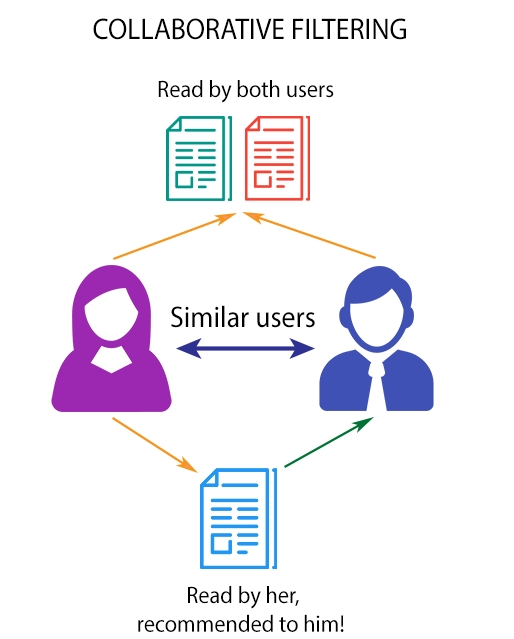
\includegraphics[max width=10cm,max height=10cm,keepaspectratio]{img_2_1}
	\caption[Filtrarea coloborativă]{Filtrarea coloborativă. Imagine preluată din \hyperlink{datameetsmedia}{[5]}.}
\end{figure} 

\subsubsection*{Filtrarea bazată pe conținut}

Filtrarea bazată pe conținut pleacă de la premisa că utiliztorii cărora le-au plăcut articole definite de anumite atribute în trecut, vor aprecia aceleași tip de articole și în viitor. Această abordare folosește atributele articolelor pentru a le compara cu profilul utilizatorilor și a oferi recomandări. Calitatea recomandărilor create folosind această strategie este influențată de setul de atribute ales pentru articole.

Similar cu filtrarea coloborativă și filtrarea bazată pe conținut prezintă dezavantaje în momentul în care în sistem intră un nou utilizator fără istoric \hyperlink{ErionCanoMaurizioMorisio}{[4]}.

\begin{figure}[!h]
	\centering
	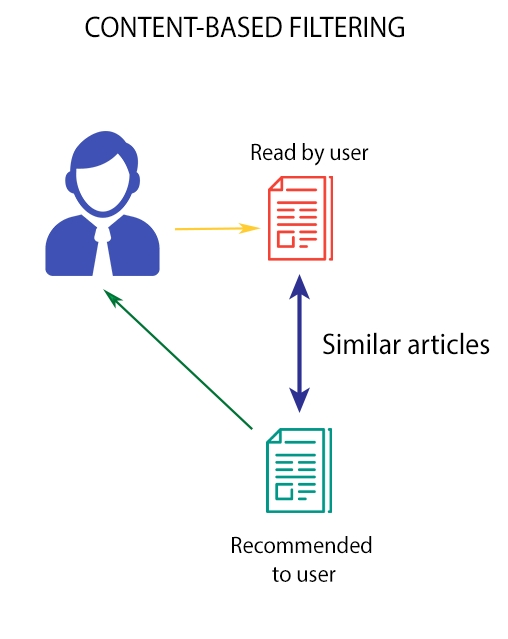
\includegraphics[max width=10cm,max height=10cm,keepaspectratio]{img_2_2}
	\caption[Filtrarea bazată pe conținut]{Filtrarea bazată pe conținut. Imagine preluată din \hyperlink{datameetsmedia}{[5]}.}
\end{figure} 

\subsubsection*{Filtrarea demografică}

Filtrarea demografică folosește atribute precum vârsta, genul, educația, etc. pentru a identifica categoriile de utilizatori. Nu prezintă dezavantaje atunci când apar noi utilizatori în sistem și nu se folosește de ratinguri, sau alt sistem de feedback, pentru a face recomandări.

Dezavantajul este reprezentat de faptul că procesul de colectare al datelor demografice poate fi îngreunat de legislație fapt ce reprezintă o limitare a acestei metode \hyperlink{ErionCanoMaurizioMorisio}{[4]}.

\subsubsection*{Filtrarea bazată pe cunoștințe}

Filtrarea bazată pe cunoștințe folosește cunoștințele despre utilizatori și articole pentru a spune ce articole îndeplinesc cerințele utilizatorilor și genereaza recomandări în consecință. Filtrare bazată pe cunoștințe are la bază constrângeri și este capabilă să recomande chiar și articole complexe care nu sunt cumpărate atât de des, precum mașini sau case \hyperlink{ErionCanoMaurizioMorisio}{[4]}.

\subsection{Funcții de loss}

\subsubsection*{BPR: Bayesian Personalised Ranking}

Maximizează diferența de predicției dintre un exemplu pozitiv și un exemplu negativ ales aleator. Este utilă atunci când sunt prezente doar interacțiuni pozitive și se dorește optimizarea acurateții \hyperlink{lighfm}{[6]}.

\subsubsection*{WARP: Weighted Approximate-Rank}

Maximizează rangul exemplelor positive prin eșantionarea repetată a exemplelor negative până când se constată o încălcare a rangului. Este utilă atunci când sunt prezente doar interacțiuni pozitive și se dorește optimizarea preciziei@k \hyperlink{lighfm}{[6]}.

\section{Rețele neurale convoluționale}

\subsection{Noțiuni generale}

Rețelele neurale convoluționale sunt foarte similare cu rețelele neurale fiind formate din neuroni ce învață ponderi ($w$) și baiasuri ($b$). Scopul rețelei convoluționale este de a primi o imagine la input și de a scoate la output un scor pentru fiecare clasă ce corespunde imaginii. 

Spre exemplu, la input se dă o imagine cu un autovehicul, iar rețeaua convoluțională poate spune că în imagine este o mașină în proporție de 80\%, un camion în proporție de 10\%, un avion în proporție de 6\%, o barcă în proporție de 3\% sau un cal în proporție de 1\%.

\begin{figure}[!h]
	\centering
	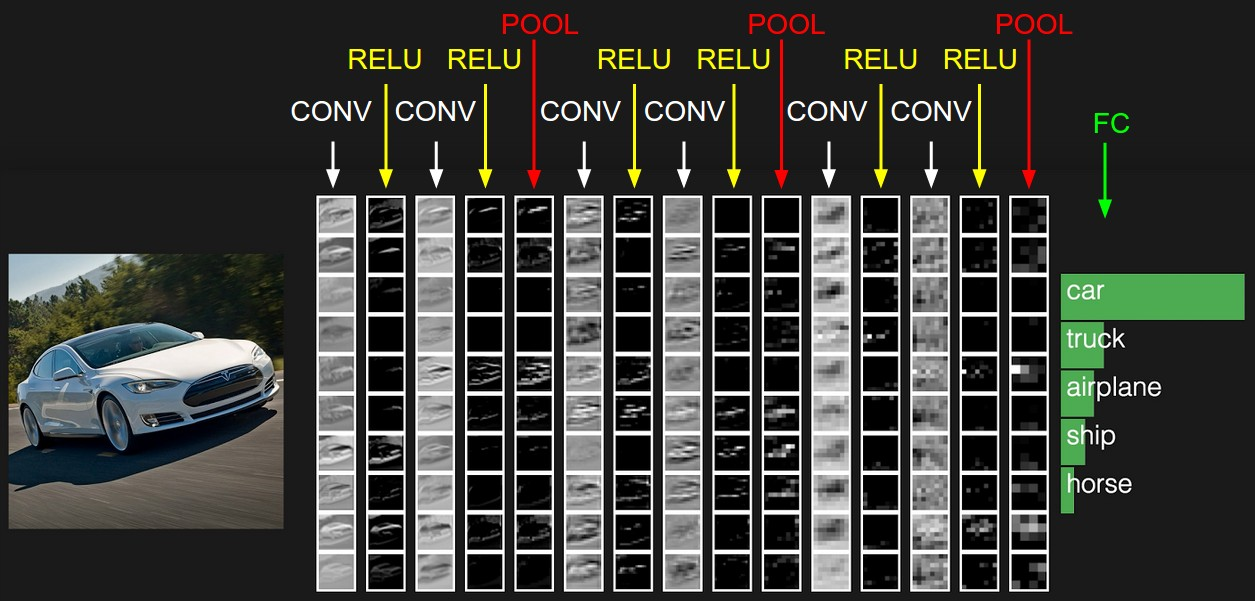
\includegraphics[max width=10cm,max height=10cm,keepaspectratio]{img_2_3}
	\caption[Exemplu rețea convoluțională]{Exemplu de rețea convoluțională care primește la input o imagine și produce la output o listă de clase ce pot descrie imaginea de input. Imagine preluată din \hyperlink{datameetsmedia}{[7]}.}
\end{figure} 

Rețelele convoluționale sunt compuse dintr-o secvență de layere ce poate fi împărțită în trei tipuri principale de layere \hyperlink{cs231n}{[7]}:

\begin{enumerate}
  \item Convolutional Layer este layerul de bază într-o rețea convoluțională. Parametrii acestui layer sunt reprezentați de filtre învățabile, unde fiecare filtru reprezintă o mică bucată din imaginea de input. De exemplu, un filtru pentru pentru acest layer poate avea dimensiunea de $5\times5\times3$, dimensiune ce reprezintă faptul că se iau 5 pixeli pe lațime și înălțime cu o adâncime de 3, unde adâncimea reprezintă canalele RGB. În continuare se glisează fiecare filtru peste input și se compune produsul dintre filtre și input la fiecare poziție. În urma acestei operații se produce un vector de activare 2-dimensional care reprezintă răspunsul filtrului la fiecare poziție. Altfel spun, rețeaua va învăța filtre care se activează atunci când sunt prezente anumite tipuri de caracteristici, precum culoarea sau orientarea.

\begin{figure}[!h]
	\centering
	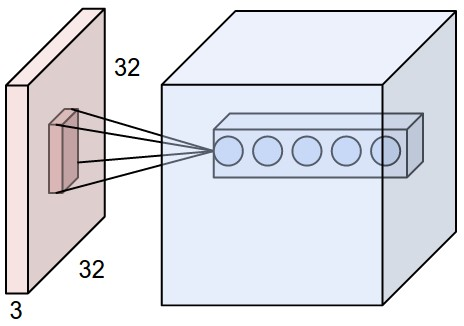
\includegraphics[max width=10cm,max height=10cm,keepaspectratio]{img_2_4}
	\caption[Exemplu de filtru aplicat peste input]{Exemplu de filtru aplicat peste input într-un layer convoluțional. Imagine preluată din \hyperlink{datameetsmedia}{[7]}.}
\end{figure}   
  
  \item Pooling Layer reprezintă o practică des folosită între mai multe layere convoluționale succesive. Această operație reduce numărul de parametrii (dimensiunea), computațiile din rețea și controlează overfittingul. Se execută indepedent pe fiecare nivel al adâncimii unui input și pastrează valoarea maximă a acelei zone. Rezultatul este o zonă de caracteristicii mai mică dar care păstrează cea mai relevantă statistică.

\begin{figure}[!tbp]
  \begin{subfigure}[b]{0.4\textwidth}
    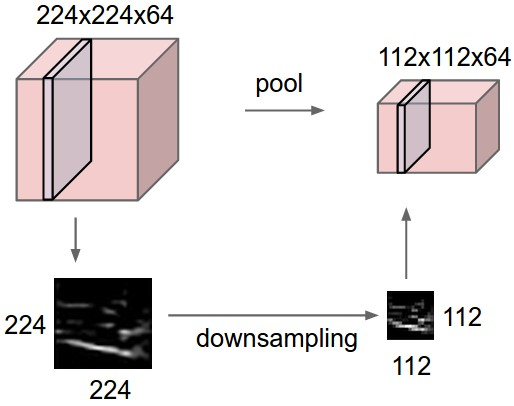
\includegraphics[width=\textwidth]{img_2_5}
    \caption{Reducerea dimensiunii.}
    \label{fig:f1}
  \end{subfigure}
  \hfill
  \begin{subfigure}[b]{0.4\textwidth}
    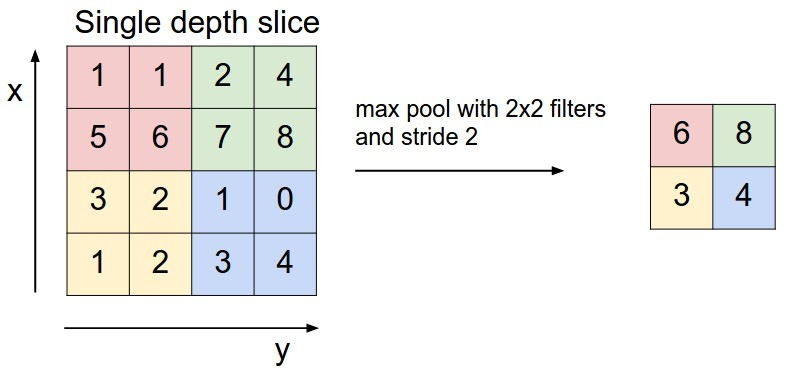
\includegraphics[width=\textwidth]{img_2_6}
    \caption{Filtrul de $2\times2$ aplicat ce păstrează valoarea maximă.}
    \label{fig:f2}
  \end{subfigure}
  \caption[Exemplu de pooling]{Exemplu de pooling. Imagine preluată din \hyperlink{datameetsmedia}{[7]}.}
\end{figure}
  
  \item Fully-Connected Layer este stratul în care caracteristicile sunt vectorizate pentru a putea fi folosite.
\end{enumerate}

\subsection{VGG}

\subsection{InceptionV3}

\subsection{ResNet}

\subsection{NASNet}



\section{Clustere}

\subsection{Noțiuni generale}

\subsection{K-nearest neighbors}
